\section{Results and Discussion}\label{sec:results}

This chapter first presents the results of the two image-analysis stages and then the evaluation of the domain-expert LLM, which is the central question of the thesis topic. It continues with an end-to-end case study of a real run of the lab assistant, and ends with a discussion of the research questions and the limitations.

\subsection{Stage 1: detection results}

On the 126-image TXL-PBC test split, the detector reached a mAP@0.50 of 0.985 and a mAP@0.50:0.95 of 0.876 (Table~\ref{tab:det}). White cells were found with a recall of 1.000, so every annotated white cell in the test split reaches the classifier. Red cells have the lowest recall (0.943), as expected for densely packed, overlapping cells, and platelets --- the smallest and rarest objects (49 test instances) --- have the lowest precision and mAP. The normalised confusion matrix is nearly diagonal; the errors are missed cells and false detections against the background rather than confusions between classes (Figure~\ref{fig:det}). The training and validation losses decreased steadily over the 50 epochs and the validation metrics levelled off without a late decline, so there is no sign of over-fitting (Figure~\ref{fig:yolo-curves}).

\begin{table}[H]
\centering
\caption{YOLOv8s results on the TXL-PBC test split.}
\label{tab:det}
\small
\begin{tabular}{lrrcccc}
\toprule
\textbf{Class} & \textbf{Images} & \textbf{Instances} & \textbf{Precision} & \textbf{Recall} & \textbf{mAP@0.50} & \textbf{mAP@0.50:0.95} \\
\midrule
WBC & 126 & 131 & 0.992 & 1.000 & 0.995 & 0.889 \\
RBC & 126 & 1{,}688 & 0.977 & 0.943 & 0.990 & 0.906 \\
Platelet & 34 & 49 & 0.958 & 0.939 & 0.970 & 0.834 \\
\midrule
\textbf{All} & 126 & 1{,}868 & \textbf{0.976} & \textbf{0.961} & \textbf{0.985} & \textbf{0.876} \\
\bottomrule
\end{tabular}
\end{table}

\begin{figure}[H]
\centering
\begin{subfigure}[t]{0.62\textwidth}\centering
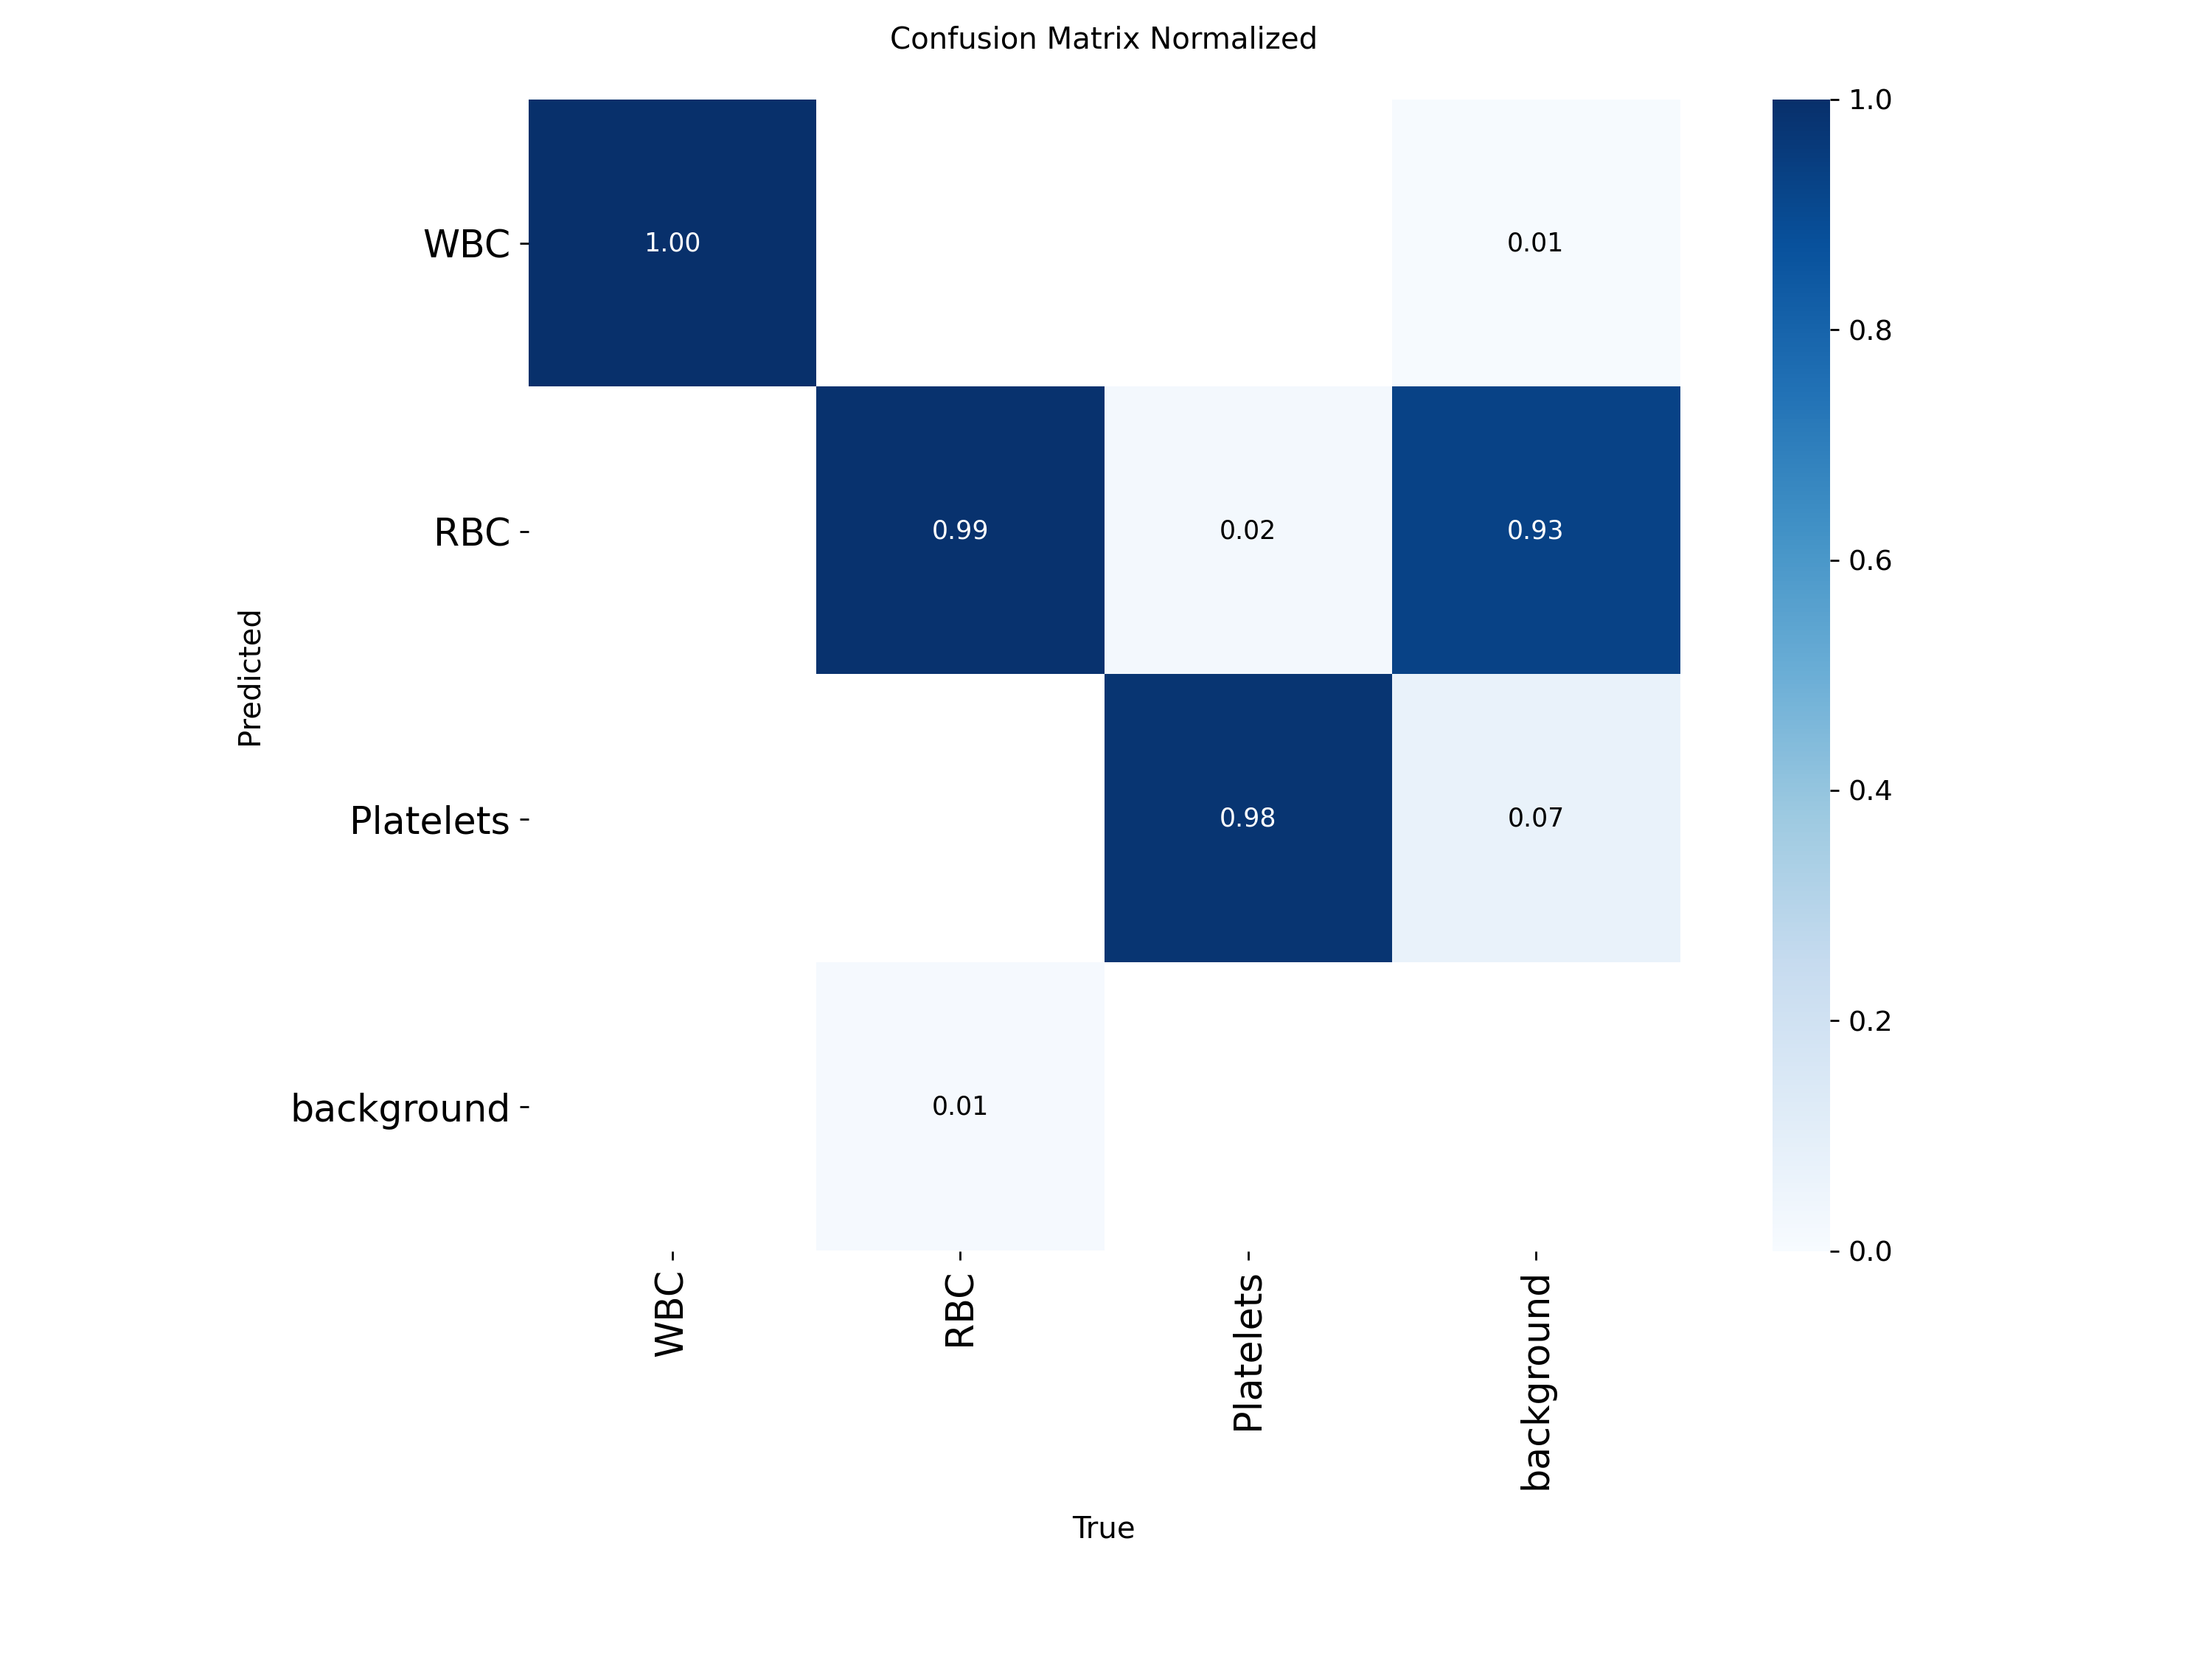
\includegraphics[width=\textwidth]{figures/stage1_results_confusion_matrix.png}
\caption{Normalised confusion matrix.}
\end{subfigure}\\[6pt]
\begin{subfigure}[t]{\textwidth}\centering
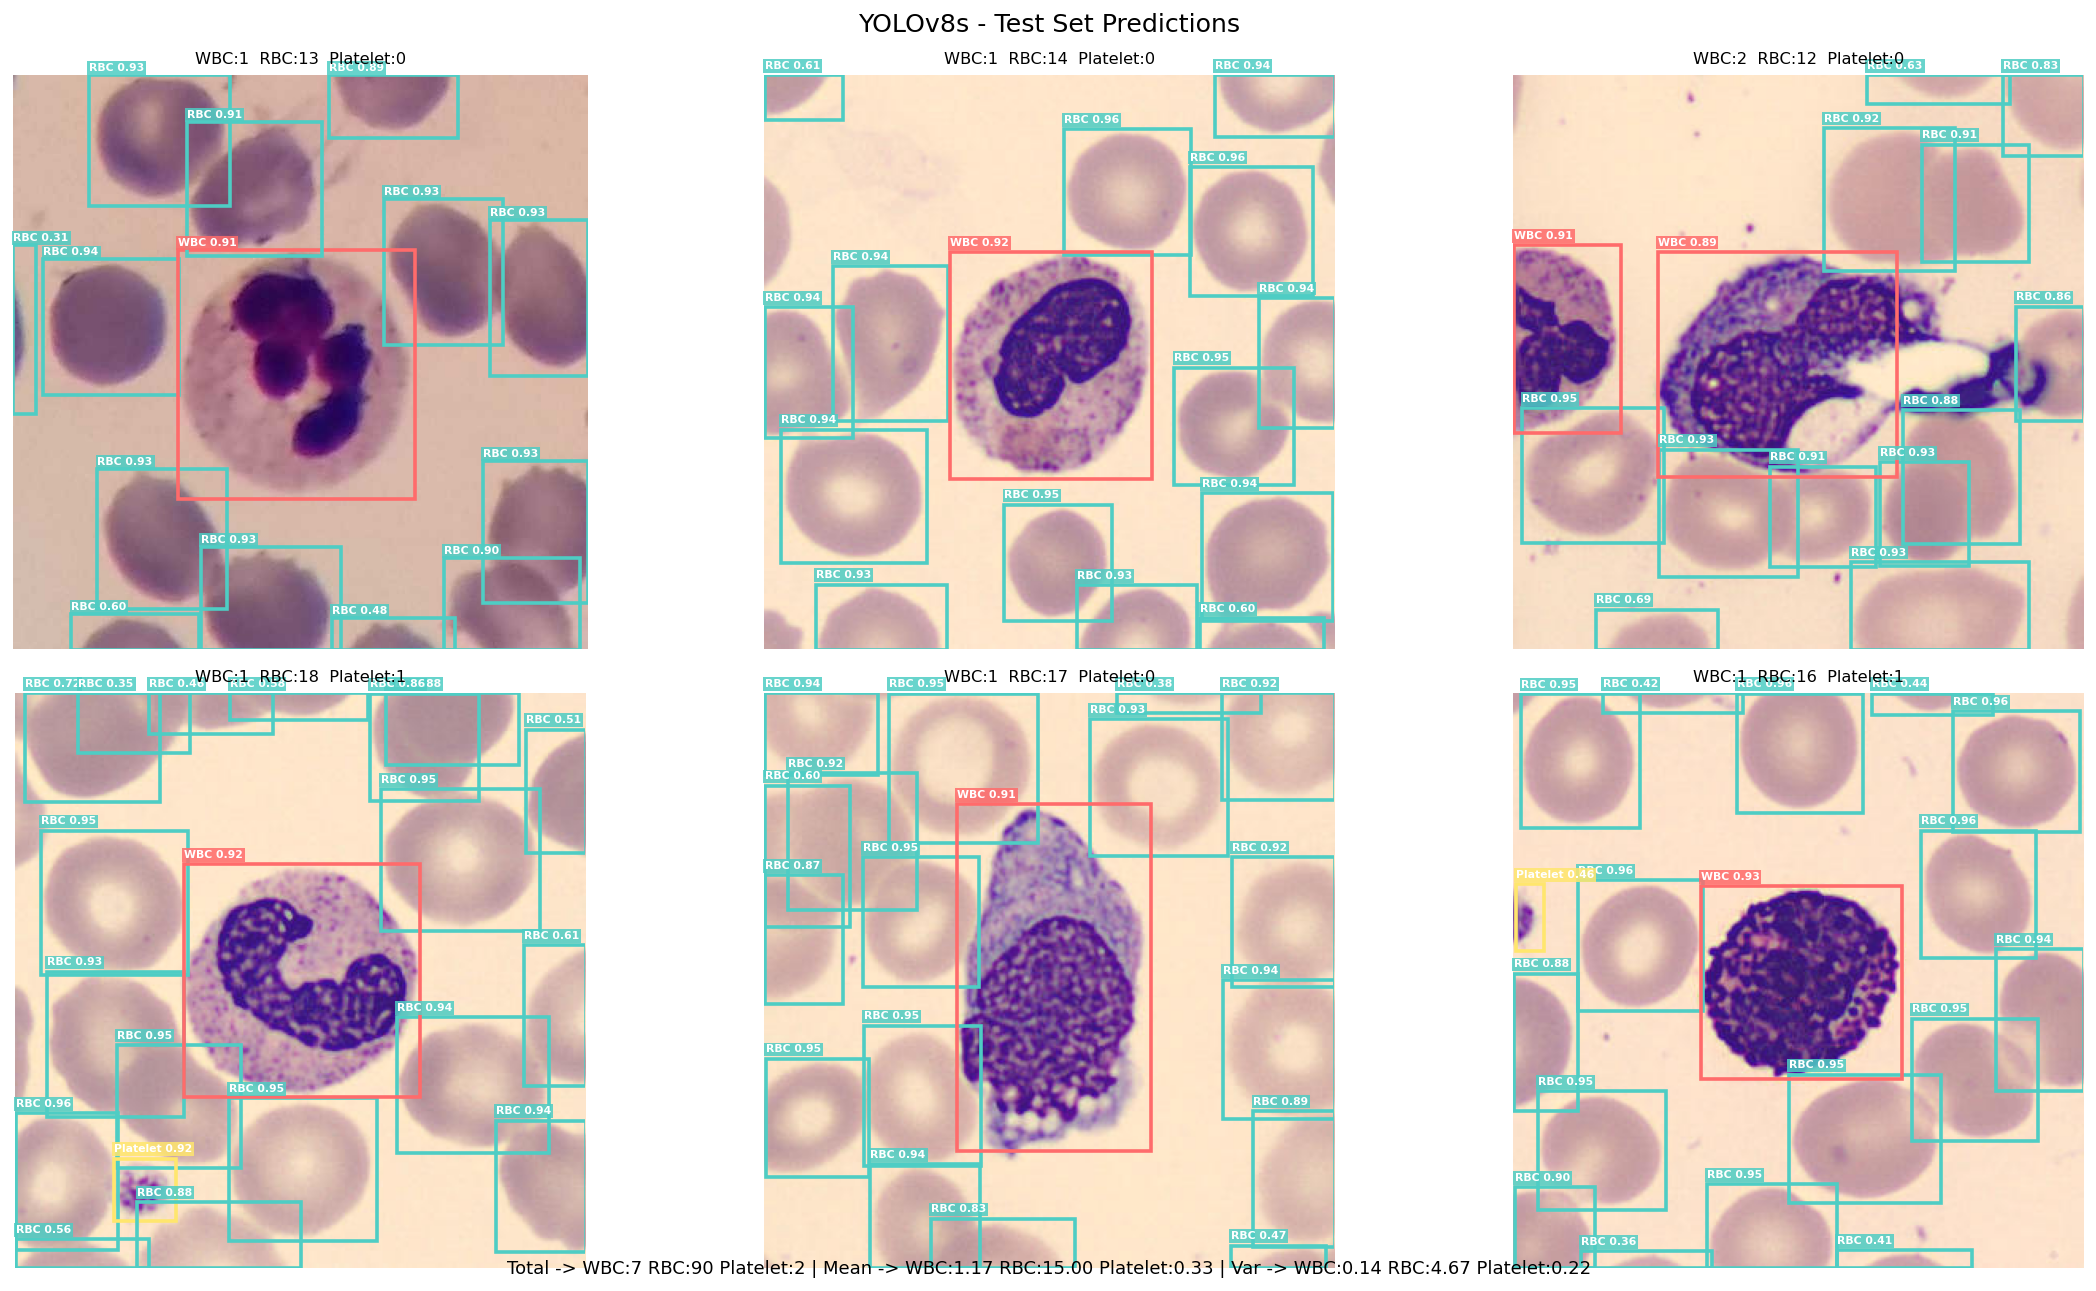
\includegraphics[width=0.9\textwidth]{figures/stage1_results_predictions.png}
\caption{Predictions on test images.}
\end{subfigure}
\caption{Detection results on the TXL-PBC test split.}
\label{fig:det}
\end{figure}

\begin{figure}[H]
\centering
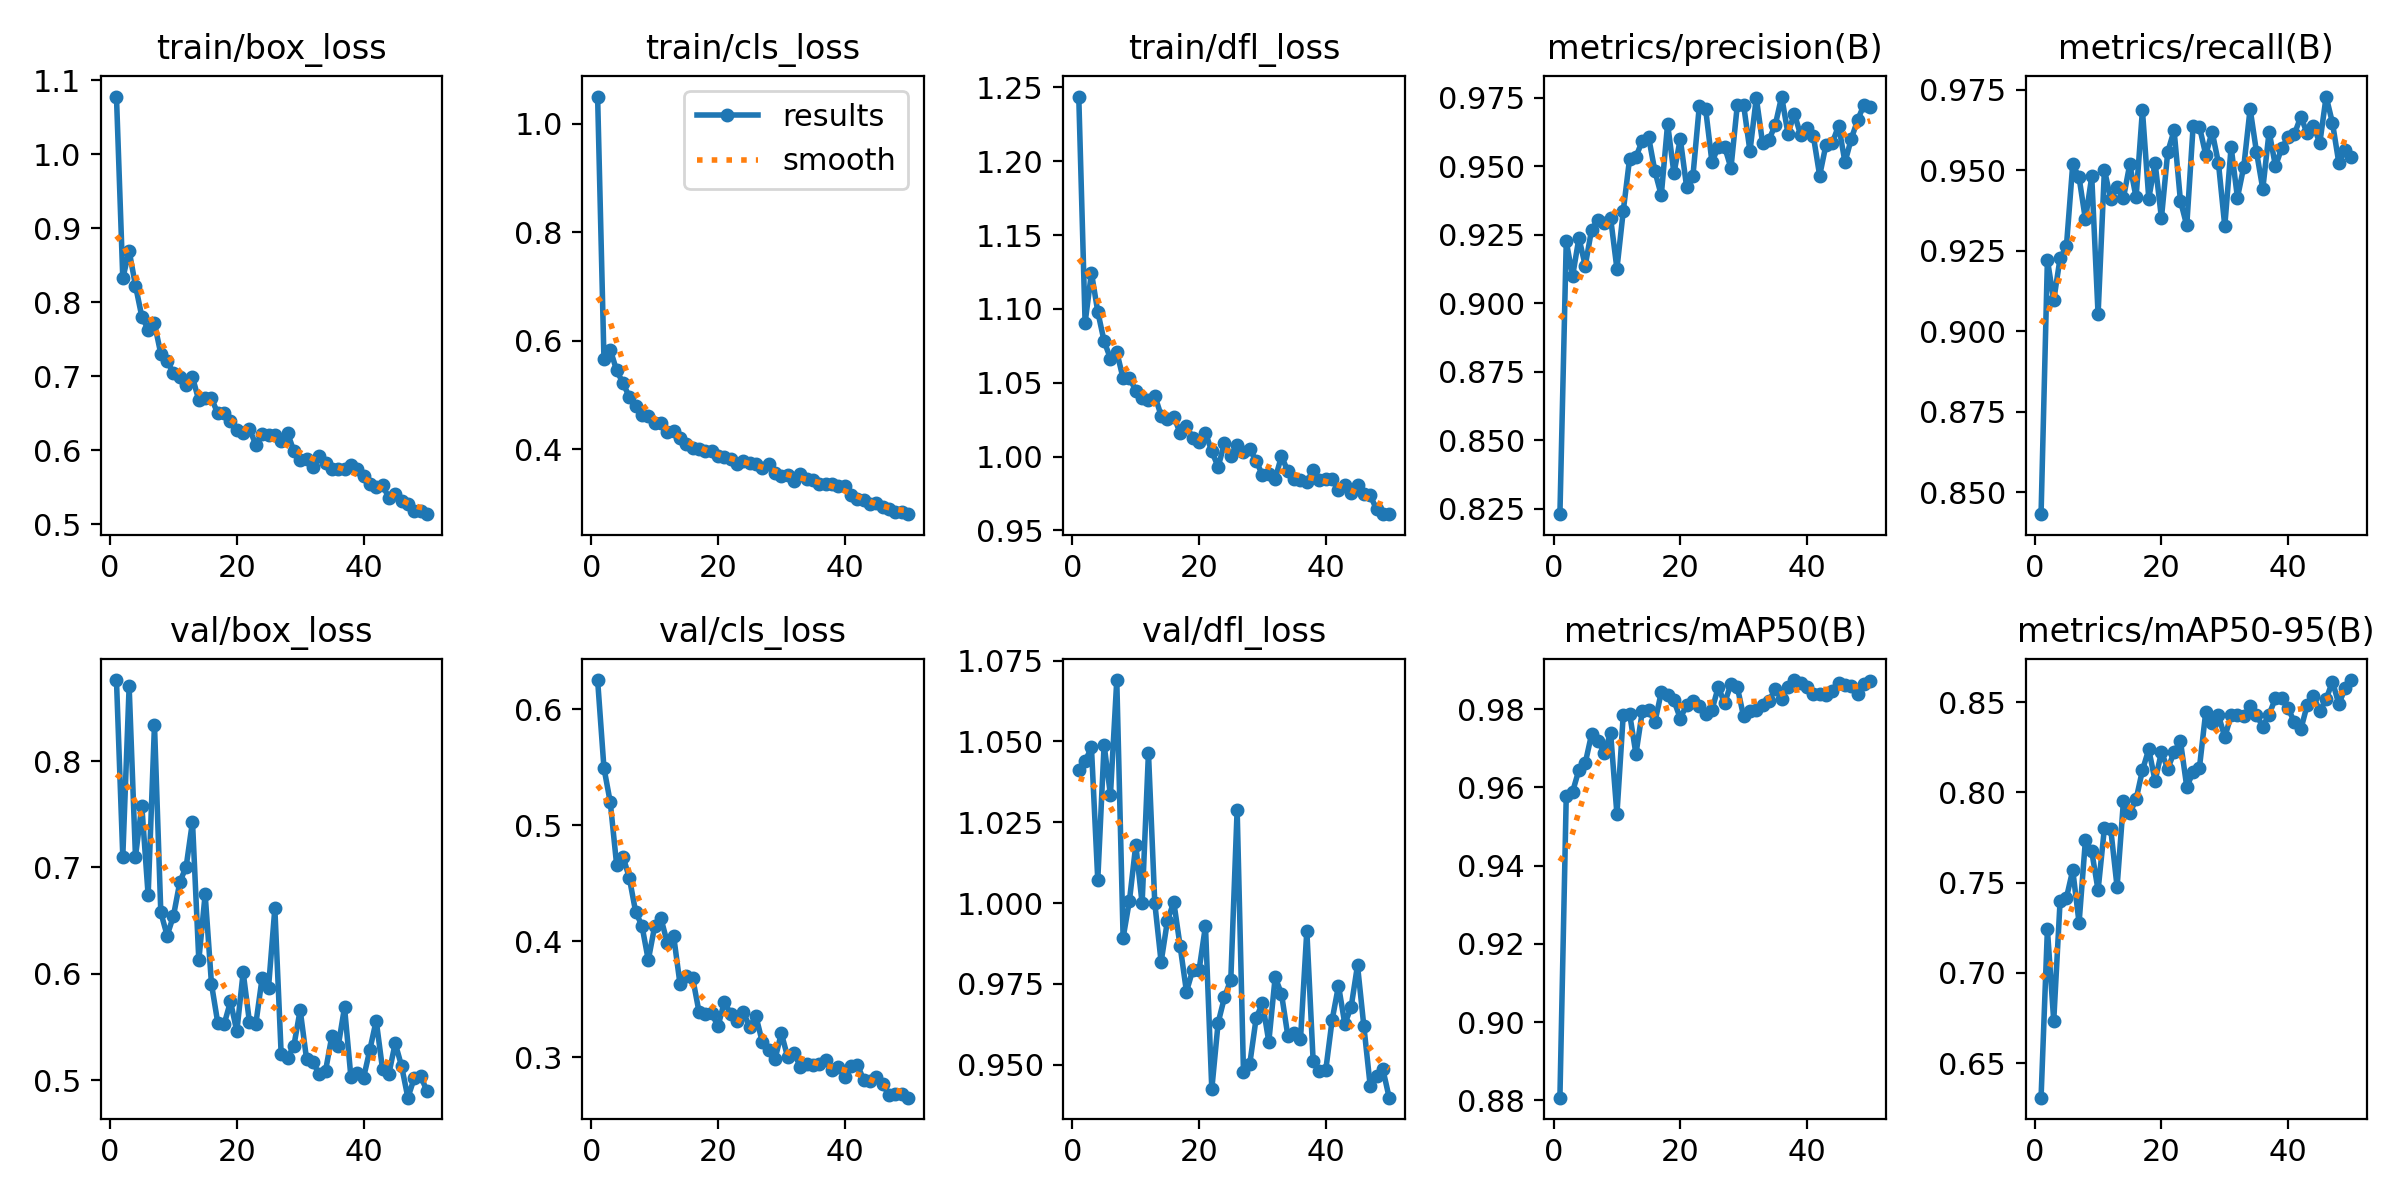
\includegraphics[width=\textwidth]{figures/stage1_results_training_curves.png}
\caption{YOLOv8s training curves over 50 epochs: training and validation box, class and distribution-focal losses (left three columns) and validation precision, recall, mAP@0.50 and mAP@0.50:0.95 (right).}
\label{fig:yolo-curves}
\end{figure}

\subsection{Stage 2: classification and uncertainty results}

The saved EfficientNet-B0 checkpoint reached a top-1 accuracy of \textbf{99.44\,\%} on the 3{,}419 PBC test images (macro-averaged F1 0.99). Per-class results are in Table~\ref{tab:cls} and the confusion matrix in Figure~\ref{fig:cls}. The only class below 0.99 recall is the immature granulocyte (0.98), whose errors go to neutrophils (0.02) and erythroblasts (0.01). This is morphologically plausible: immature granulocytes are transitional forms between myeloid precursors and mature neutrophils, and the boundary is also difficult for human reviewers. It is exactly the kind of case in which an uncertainty estimate is useful.

Freezing the backbone limited Phase~1 to a best monitored accuracy of 88.97\,\%; unfreezing it in Phase~2 raised this to 98.65\,\% within eight epochs, showing that adapting the pre-trained features is essential for fine-grained cell morphology. The final evaluation of the saved checkpoint, in a later notebook cell, gave 99.44\,\% on the same images; the difference between the two numbers was not investigated and suggests that the saved checkpoint is not exactly the one monitored in the displayed training log. Together with the caveat in Section~\ref{sec:method} --- the test images were also used for model selection --- this means that 99.44\,\% should be read as an optimistic estimate.

\begin{table}[H]
\centering
\caption{Per-class results of EfficientNet-B0 on the PBC test split (scikit-learn classification report).}
\label{tab:cls}
\small
\begin{tabular}{lcccr}
\toprule
\textbf{Class} & \textbf{Precision} & \textbf{Recall} & \textbf{F1} & \textbf{Support} \\
\midrule
Basophil & 1.00 & 1.00 & 1.00 & 237 \\
Eosinophil & 1.00 & 1.00 & 1.00 & 620 \\
Erythroblast & 0.98 & 1.00 & 0.99 & 309 \\
Immature granulocyte & 1.00 & 0.98 & 0.99 & 598 \\
Lymphocyte & 0.99 & 1.00 & 0.99 & 256 \\
Monocyte & 1.00 & 0.99 & 1.00 & 286 \\
Neutrophil & 0.98 & 1.00 & 0.99 & 649 \\
Platelet & 1.00 & 1.00 & 1.00 & 464 \\
\midrule
\textbf{Accuracy} & \multicolumn{3}{c}{\textbf{0.9944}} & 3{,}419 \\
\bottomrule
\end{tabular}
\end{table}

\begin{figure}[H]
\centering
\begin{subfigure}[t]{0.66\textwidth}\centering
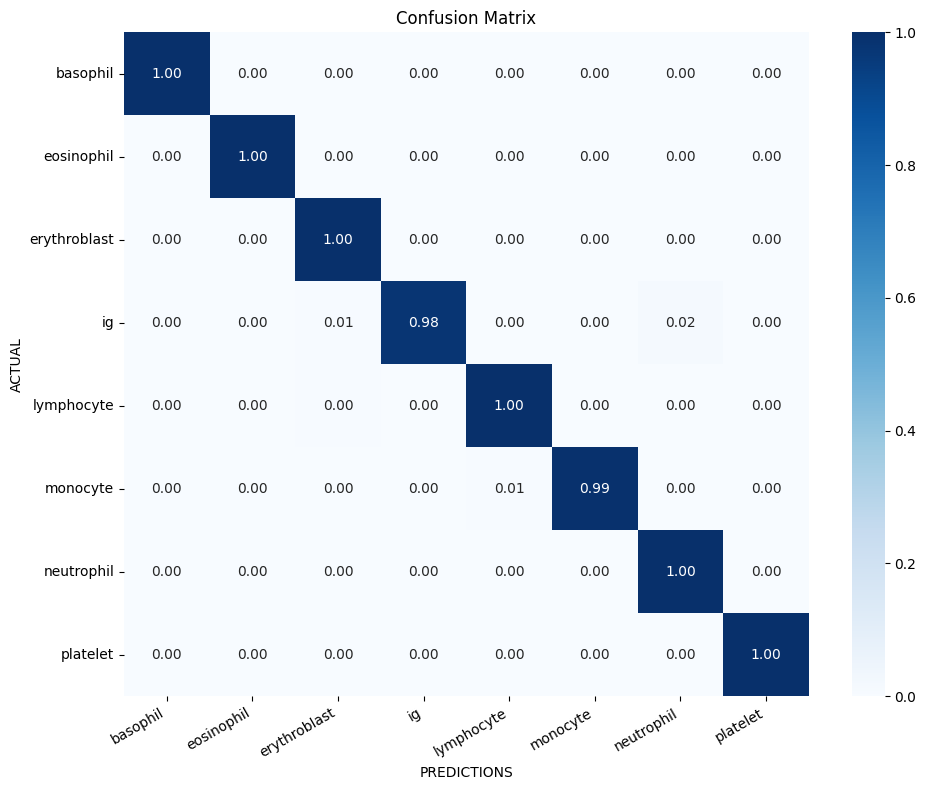
\includegraphics[width=\textwidth]{figures/stage2_embedded_confusion_matrix_test.png}
\caption{Normalised confusion matrix of the saved checkpoint.}
\end{subfigure}\\[6pt]
\begin{subfigure}[t]{\textwidth}\centering
\includegraphics[width=\textwidth]{figures/effnet_training_curves.pdf}
\caption{Loss and accuracy over both training phases, re-plotted from the notebook's training log. The ``monitored'' curve was computed on the test partition (see the caveat in Section~\ref{sec:method}).}
\end{subfigure}
\caption{Classification results on the PBC test split.}
\label{fig:cls}
\end{figure}

\begin{figure}[H]
\centering
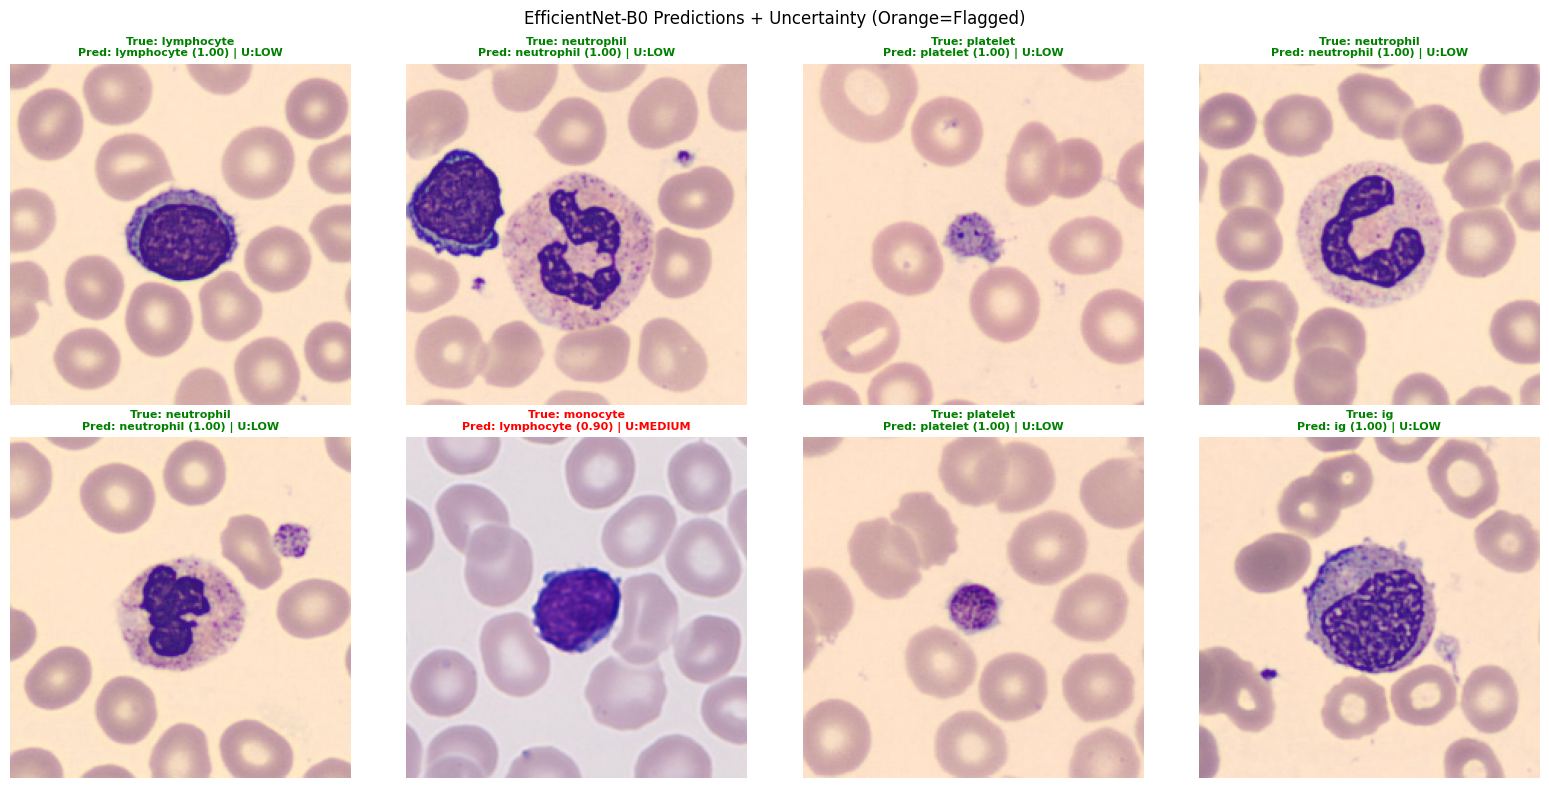
\includegraphics[width=0.9\textwidth,height=7cm,keepaspectratio]{figures/stage2_embedded_mc_dropout_uncertainty_demo.png}
\caption{MC-Dropout predictions on eight test images. The seven correct predictions receive the uncertainty level LOW; the one error (a monocyte predicted as a lymphocyte with confidence 0.90, red title) receives MEDIUM. MEDIUM is not flagged, so this error would not by itself trigger expert review.}
\label{fig:mc}
\end{figure}

\paragraph{An example of domain shift.} The PBC images used for training come from a single analyser with standardised staining. Figure~\ref{fig:shift} shows the combined Stage~1 + Stage~2 output on an image from a different source, produced in the Stage-3 notebook. The white cell has a segmented nucleus and granular cytoplasm, the appearance of a mature granulocyte, yet the classifier labelled it \emph{erythroblast} with a probability of 0.90. This single example does not measure the size of the problem, but it illustrates why the benchmark accuracy should not be expected to transfer unchanged to smears from other laboratories.

\begin{figure}[H]
\centering
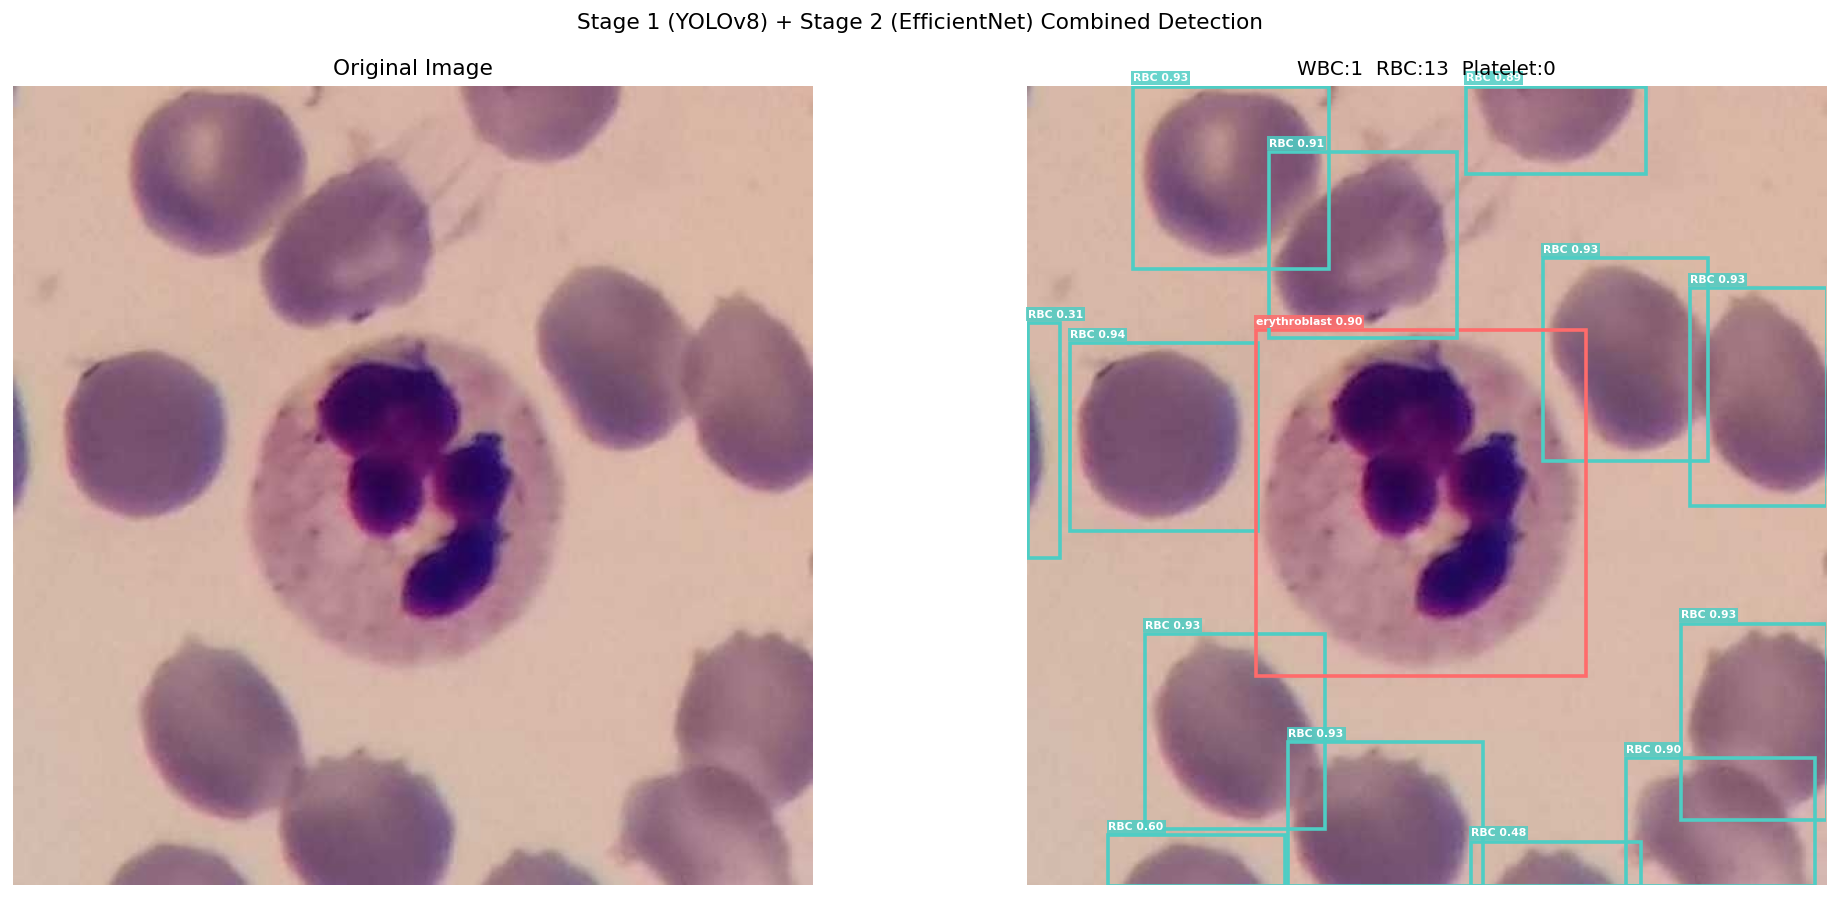
\includegraphics[width=0.9\textwidth]{figures/stage3_results_pipeline_output.png}
\caption{Stage 1 + Stage 2 output on an image from outside the training distribution: 13 red cells and one white cell were detected; the white cell, which appears to be a segmented granulocyte, was classified as \emph{erythroblast} (0.90). (This notebook run used a lower detection threshold than the 0.50 of the final system, so some low-confidence red-cell boxes are shown.)}
\label{fig:shift}
\end{figure}

No calibration study was performed: the thesis does not report whether cells marked HIGH uncertainty are more often misclassified. MC-Dropout is therefore used as a practical signal that makes difficult cells visible, not as a validated error predictor.

\subsection{Quantitative evaluation of the domain expert}\label{sec:res-de}

Table~\ref{tab:de} and Figure~\ref{fig:de} summarise the comparison of the base model, the fine-tuned model and GPT-4o.

\begin{table}[H]
\centering
\caption{Domain-expert evaluation. In-domain metrics are means over 100 held-out textbook questions; MedMCQA accuracy is over 100 hematology-related exam questions (not run for GPT-4o). Best value per column in bold.}
\label{tab:de}
\small
\begin{tabular}{lccccc}
\toprule
 & \multicolumn{4}{c}{\textbf{In-domain held-out questions}} & \textbf{External} \\
\cmidrule(lr){2-5}\cmidrule(lr){6-6}
\textbf{System} & \textbf{Sem.\ sim.} & \textbf{ROUGE-L} & \textbf{Source marker} & \textbf{Words} & \textbf{MedMCQA} \\
\midrule
Llama-3.1-8B (base) & 0.752 & 0.161 & 7\,\% & 158.5 & 56\,\% \\
Llama-3.1-8B + QLoRA (ours) & \textbf{0.831} & \textbf{0.433} & 100\,\% & 39.4 & \textbf{57\,\%} \\
GPT-4o (reference) & 0.774 & 0.181 & 88\,\% & 159.9 & -- \\
\midrule
Reference answers & -- & -- & 100\,\% & 39.2 & -- \\
\bottomrule
\end{tabular}
\end{table}

\begin{figure}[H]
\centering
\includegraphics[width=\textwidth]{figures/domain_expert_results.pdf}
\caption{Comparison of the three systems: (a) semantic similarity and (b) ROUGE-L F1 against the textbook reference answers on 100 held-out questions; (c) accuracy on 100 hematology-related MedMCQA questions, with the 25\,\% chance level.}
\label{fig:de}
\end{figure}

\paragraph{In-domain questions.} Fine-tuning brought the model's answers much closer to the textbook reference answers. ROUGE-L rose from 0.161 to 0.433; the paired bootstrap 95\,\% confidence interval of the improvement is $[0.252,\ 0.293]$, and the fine-tuned model scored higher than the base model on \emph{every one} of the 100 questions. Semantic similarity rose from 0.752 to 0.831. On both measures the fine-tuned 8-billion-parameter model also exceeded GPT-4o (ROUGE-L difference $+0.252$, 95\,\% CI $[0.234,\ 0.273]$). Its answers are about four times shorter than those of the other two systems (39 vs.\ 159 words) and match the length of the reference answers (39 words).

These numbers must be read carefully. The reference answers were written by a GPT model from the textbook passages, in a particular concise style, and the fine-tuned model was trained on 1{,}890 answers in exactly that style. Part of the gain is therefore a gain in \emph{form}: length, wording and structure. ROUGE-L rewards this strongly; semantic similarity, which is less sensitive to wording, shows a smaller but still clear gain. GPT-4o's lower scores do not mean that its answers are less correct --- it writes longer, more general explanations that overlap less with the short reference text.

\paragraph{External questions.} On the MedMCQA questions the fine-tuned model answered 57 of 100 correctly and the base model 56. The two models disagreed on 21 questions (base correct only: 10; fine-tuned correct only: 11), and the exact McNemar test gives $p = 1.0$: there is no evidence of a difference. Fine-tuning on 1{,}890 textbook pairs neither improved nor damaged the model's general hematology knowledge. (Both models are well above the 25\,\% chance level; three of the base model's answers could not be parsed as a letter and count as wrong.)

\paragraph{Interpretation.} Together, the two results give a clear picture: \emph{QLoRA fine-tuning taught the model how the domain expert should answer --- concisely, in the textbook's terminology and with a source line --- but it did not teach it new medical knowledge.} This agrees with the literature, which finds that retrieval is more effective than fine-tuning for injecting knowledge \cite{ovadia2024}, and it supports the design choice of building the runtime expert around retrieval and tools.

\subsection{Qualitative analysis: citations and errors}

\paragraph{Invented citations in the base model.} No source was given to the models, yet the base Llama model named a specific textbook, author or edition in \textbf{52 of the 100} in-domain answers. Typical openings were:

\begin{quote}\small
``According to the textbook \emph{`Hematology: A Very Short Introduction'} by Valerie Higgs [1] \ldots'' \\
``According to the textbook \emph{`Hematopathology'} by Knowles, 2nd edition, [Reference 1] \ldots''
\end{quote}

The attributions are fabricated --- the model was never shown these books, and in several answers the same title is attributed to different authors --- but they look convincing. This is the failure mode described by Walters and Wilder for ChatGPT \cite{walters2023}, and it is caused here by the system prompt, which asks the model to ``cite'' a ``provided textbook reference'' that is not there. Neither the fine-tuned model nor GPT-4o named an invented book. GPT-4o, however, inserted a bare ``[Reference~1]'' marker in 32 answers, pointing to a reference that did not exist --- a milder form of the same behaviour.

\paragraph{Uniform source lines in the fine-tuned model.} The fine-tuned model ended \emph{every} answer with a source line (100\,\% in Table~\ref{tab:de}), naming the first textbook in 92 answers and the second in 8. It usually chose the right book --- five of the seven questions from the second book were labelled correctly --- which shows that it learned which topics belong to which book. But the line is learned format, not provenance: the model attaches it to correct and incorrect answers alike. Examples of incorrect answers that carry the source line are:

\begin{itemize}
  \item \emph{Pure red cell aplasia}: the model expects ``macrocytic red cells'', whereas the reference answer describes a normocytic normochromic anaemia with reticulocytopenia.
  \item \emph{Hypertransfusion in thalassaemia}: the model states a target haemoglobin ``above 14\,g/dl''; the reference answer gives 9.5--10\,g/dl.
  \item \emph{Myeloblast vs.\ lymphoblast} (qualitative question): the model describes the myeloblast as having ``coarse nuclear chromatin'' and ``2--3 large, bright blue, specific granules'', which is incorrect --- myeloblasts typically have fine chromatin and few or no granules.
\end{itemize}

The fine-tuned model therefore looks more authoritative than the base model while being no more knowledgeable. For a domain expert this is an important and somewhat uncomfortable finding: \textbf{a citation produced by a language model is not evidence}. A citation is only useful if it points to a passage that was actually retrieved and can be opened, as in the RAG agent, where every \code{[Reference N]} corresponds to a logged tool result.

\paragraph{Clinical scenarios.} Table~\ref{tab:qual} summarises the answers to the five hand-written clinical questions. Both models recognise the typical patterns (neutrophilic leukocytosis with toxic granulation suggests infection or inflammation; a microcytic anaemia with target cells suggests a hemoglobinopathy). The fine-tuned model is shorter and more decisive; the base model is longer, lists more possibilities, and often decorates its answer with invented reference numbers.

\begin{table}[H]
\centering
\caption{Condensed answers to the five clinical questions (full answers in \code{evaluation\_report.json}).}
\label{tab:qual}
\footnotesize
\begin{tabularx}{\textwidth}{>{\raggedright\arraybackslash}p{3.3cm} X X}
\toprule
\textbf{Question} & \textbf{Base model} & \textbf{Fine-tuned model} \\
\midrule
78\,\% neutrophils, toxic granulation, WBC $18 \times 10^9$/L & Leukemoid reaction or severe (bacterial) infection; long explanation & ``Neutrophilic leucocytosis with toxic granules'', suggests infection/inflammation \\
Only 2 WBCs classified (1 IG, 1 monocyte) & Classification incomplete; the differential is not representative & ``Differential unsatisfactory'' because far too few cells were counted \\
Hb 9.1\,g/dL, MCV 68\,fL, target cells & Thalassaemia, HbC, HbE, sickle cell disease, iron deficiency; Hb electrophoresis & Thalassaemia trait, sickle cell trait, Hb Lepore; solubility test for HbS (omits iron deficiency) \\
Myeloblast vs.\ lymphoblast & Mostly correct list of features & Contains factual errors (see text) \\
Platelets $90 \times 10^9$/L --- always true thrombocytopenia? & Attributes the answer to an invented textbook & ``No'' --- counts can be falsely low; correct in essence \\
\bottomrule
\end{tabularx}
\end{table}

Notably, both models --- when asked directly --- recognised that a differential based on two cells is not meaningful. As the next sections show, the full system did \emph{not} make this judgement when the same situation arose in a real run.

\subsection{End-to-end case study: an over-interpreted differential}\label{sec:case}

The saved result files in the repository contain one complete run of the system in its default configuration (GPT-4o agent) on an uploaded $640 \times 480$ smear image. It is analysed here in detail because it shows both the strengths of the design and a failure that the safety logic did not catch.

\paragraph{What the system did.} Stage~1 detected 17 red cells and \textbf{2 white cells}. Stage~2 classified one white cell as an immature granulocyte (confidence 0.955, entropy 0.216) and the other as a monocyte (confidence 0.972, entropy 0.146); both received the uncertainty level LOW, so no cell was flagged. The agent then made five tool calls: it looked up the reference ranges of immature granulocytes (0--0.5\,\%) and monocytes (2--8\,\%), read the uncertainty summary, and searched the knowledge base for ``causes of increased immature granulocytes'' and ``causes of monocytosis''. Its final report stated:

\begin{quote}\small
``The peripheral blood smear shows a significant increase in immature granulocytes (50\,\%) and monocytes (50\,\%), which is highly abnormal. [\ldots] Immature granulocytes (IG) at 50\,\%, significantly above the normal range of 0--0.5\,\% [Reference 6].'' --- Recommendation: ``Consider bone marrow biopsy if clinically indicated.'' --- \code{confidence\_assessment}: HIGH, \code{requires\_expert\_review}: \textbf{false}.
\end{quote}

\paragraph{What went wrong.} Three problems can be identified.
\begin{enumerate}
  \item \textbf{The sample was far too small.} A differential expresses each cell type as a percentage of the white cells counted. Routine manual differentials count at least 100 cells, and the reference method of CLSI H20-A2 counts several hundred \cite{clsi2007h20}. Two cells cannot establish any percentage; ``50\,\% immature granulocytes'' is an artefact of dividing by two. The system prompt told the agent that the counts are per microscope field, but it did not tell it to check the number of cells, and nothing in the code did.
  \item \textbf{A citation was misattributed.} The retrieved chunk labelled Reference~6 is about hypersegmented neutrophils in megaloblastic anaemia. The range 0--0.5\,\% actually came from the reference-range tool. The claim was correct, but its citation pointed to the wrong evidence --- the kind of error that only becomes visible because the tool trace is recorded.
  \item \textbf{The review flag stayed false.} Both cells had low MC-Dropout uncertainty, so the deterministic rule did not fire, and the model itself set the flag to false while recommending a bone-marrow biopsy. The uncertainty of the \emph{individual cells} was low; what was uncertain was the \emph{differential as a whole}, and the rule did not measure that.
\end{enumerate}

\paragraph{Lessons.} The case shows that the design choices of the thesis --- a recorded tool trace, retrieved passages that can be checked, uncertainty passed forward --- make such failures \emph{detectable}: every step above could be reconstructed from the saved output. But it also shows that per-cell uncertainty is not enough. The fix is simple and deterministic, and it has since been implemented (Section~\ref{sec:safety}): whenever fewer than a minimum number of white cells (by default 100, which in practice requires several fields of view) have been classified, the pipeline forces \code{requires\_expert\_review} to true and adds an \code{INSUFFICIENT\_CELL\_COUNT} flag, and the reasoners are told not to interpret the percentages. Applied to this case (2 cells), the rule sets the flag to true; this is covered by an automated test. The case study run itself was made before the rule existed and was not repeated. Interestingly, both language models answered correctly when asked about a two-cell differential directly (Table~\ref{tab:qual}); in the agent, the structured prompt and the tool outputs led the model to compute and interpret percentages instead. This is a strong argument for putting such domain rules into code rather than relying on the model's judgement.

\subsection{Discussion of the research questions}

\paragraph{RQ1 --- blood image classification.} Standard vision models provide strong evidence on the benchmark data: mAP@0.50 = 0.985 for detection with perfect white-cell recall, and 99.44\,\% (optimistic) classification accuracy, each classified cell carrying an uncertainty level and a Grad-CAM map. How well this transfers to smears from other laboratories was not tested.

\paragraph{RQ2 --- building the domain expert with RAG.} A general LLM was turned into a hematology expert by combining a curated textbook knowledge base, domain tools and a structured output format. The resulting agent produces interpretations with retrievable citations and a complete, auditable tool trace (Figures~\ref{fig:ui-a}--\ref{fig:ui-b}). The case study shows that this makes errors visible but does not prevent them; domain rules such as a minimum cell count must be enforced in code.

\paragraph{RQ3 --- domain fine-tuning.} QLoRA fine-tuning of Llama-3.1-8B for under an hour on a free GPU produced a model whose answers match textbook reference answers much better than those of the base model and even of GPT-4o (ROUGE-L 0.433 vs.\ 0.161 and 0.181), and which no longer invents book references. It did not improve accuracy on external exam questions (57\,\% vs.\ 56\,\%, not significant), and it learned to attach a source line regardless of correctness. Fine-tuning is therefore suitable for adapting the \emph{behaviour} of an open, self-hostable expert, but it must be combined with retrieval to supply knowledge and real provenance.

\paragraph{RQ4 --- safety and auditability.} The system passes all safety-relevant information forward and forces expert review when any cell is uncertain. The case study showed the limits of the original rule: it reacted to uncertain \emph{cells}, not to an unreliable \emph{differential}. A minimum-cell rule was therefore added. Auditability worked as intended --- the misattributed citation and the faulty reasoning could be traced step by step.

\subsection{Limitations and threats to validity}

\begin{itemize}
  \item \textbf{Synthetic reference answers.} The in-domain test answers were generated by a GPT model from the textbook, not written by hematologists. They may contain errors, and they favour a model trained on the same style. Some questions refer to ``the passage'', an artefact of the generation.
  \item \textbf{Grouping assumption in the split.} The chunk-level split assumes that consecutive records come from the same chunk, as written by the generation script; the records themselves do not store a chunk identifier.
  \item \textbf{Small, noisy external test.} The MedMCQA subset has 100 questions, about a quarter of which are only loosely related to hematology; small differences cannot be detected with this sample size.
  \item \textbf{No human or LLM-judge ratings.} Correctness was assessed with automatic similarity measures and by hand for a few answers. The planned LLM-as-judge step failed, and no clinician evaluated the answers.
  \item \textbf{Training format of the fine-tuned model.} The training examples contain no retrieved passage, so the model was not trained to read and cite evidence. The fine-tuned model was evaluated stand-alone, not inside the agent.
  \item \textbf{Classifier evaluation.} The EfficientNet test set was also used for checkpoint selection, the split is image-level rather than donor-level, and the saved checkpoint's accuracy (99.44\,\%) differs from the monitored training accuracy (98.65\,\%) without explanation. (A mismatch in the inference code, which re-created the second dropout layer with $p = 0.2$ instead of the $p = 0.3$ used in training, was found during this work and corrected; the case-study run predates the correction.)
  \item \textbf{No external validation of the vision stages.} Both vision datasets were recorded under controlled conditions; smears from other microscopes, stains or laboratories may reduce performance substantially.
  \item \textbf{Uncertainty thresholds and review rule} were set by hand and are not calibrated against error rates.
  \item \textbf{Copyright of the knowledge base.} The textbooks are copyrighted and cannot be redistributed, which limits exact reproduction of the knowledge base by others.
\end{itemize}

\clearpage
